\documentclass[../../main.tex]{subfiles}
\begin{document}
\section{Additional Tools}
A few tools remain to be explained before the algorithm can be described. These tools have a variety of reasons for being used that will be explained individually. 
\subsection{$k$-mer}
In order to create the sets that {\bf Mm½} and {\bf Mm} sketches are built with, $k$-mer will be used to partition each sequence into subsets. The $k$-mer of a sequence string are defined as follows:
\begin{center}
{\bf The $k$-mer set of a sequence string $s$ is the set of all the substrings of size $k$ of $s$.}
\end{center}
The 1-mer of a sequence string, will therefore be the set of all characters in the sequence string. It is sensible to consider the size of $k$ when partitioning sequences using $k$-mers, as the size of $k$ will determine how many $k$-mer a given character will occur in. Therefore, if two strings only differ at one character, high $k$ would mean that there would be a bigger difference between the set of $k$-mers of the one string over the other string, than at lower $k$.
\subsubsection{$k$-mer transformation}
\label{sec:kmertransformation}

Given that the $k$-mers will be used as hash function input, it is reasonable to transform them to an input that is easy to map. As sequence strings are only comprimised of 4 characters (A,C,G,T), each character is assigned a 2 bit value so that $A=\mathbf{00},C=\mathbf{01},G=\mathbf{10},T/U=\mathbf{11}$, and then put them in sequence according to their position in the substring, eg.
\begin{figure}[h]
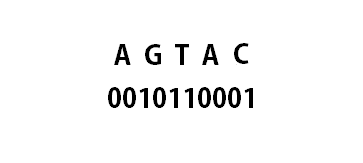
\includegraphics[scale=0.4]{fig/kmertransformed}
\end{figure}\\
which also reduces the memory usage by 75\% .
\subsection{MapReduce}\label{sec:mapreduce}
Given a sizeable amount of sequences per file, it is often advantageous to have a programming model which could parallelize and distribute the task. For this purpose, MapReduce is a popular programming model. It works by distributing its task to a multitude of workers, which can be either computers or cores. It expresses its computation as two functions:
\begin{enumerate}
\item Map: Runs a function over each element of a list and returns an intermediate value.
\item Reduce: Merges the intermediate values to form a potentially smaller set of values.
\end{enumerate}

As explained in~\cite{mapreduceExplained}, MapReduce processes input by the following steps
\begin{enumerate}
\item Map step: Splits the input into $M$ splits. Each split is then distributed to a worker who will perform a Map function on the given split and saves the result into a temporary storage.
\item Shuffle step: The results from the Map calls are then written to a local disk, partitioned into $R$ regions.
\item Reduce step: For each region, a worker is set to run a Reduce job on it, in parallel.
\end{enumerate}

Since MapReduce splits the input to several smaller parts, as long as one uses a MapReduce operation it is not possible to exceed the memory of the computer. MapReduce has been shown to scale better than other parallel programming tools for input sizes that surpass 100 Mb, which is why it chosen~\cite{compForkMapRed}. However, MapReduce has been shown to be very slow at small input files~\cite{compForkMapRed}, because of startup time and a difficulty of partitioning small files. The open source Apache Hadoop MapReduce distribution was used for this project. 

\subsection{Levenshtein Distance}\label{sec:levenshtein}
For a precise distance metric between two string, the Levenshtein distance is quite applicable. Given two strings, $s_1$ and $s_2$, the \textbf{Levenshtein distance} is defined as the minimum number of single character edits necessary to change $s_1$ into $s_2$. The \textbf{Levenshtein similarity} could then be calculated as
\begin{equation}\label{levenshteindistance}
sim=\frac{\max(s_1,s_2) - \mathrm{LevenshteinDistance}(s_1,s_2)}{\max(s_1,s_2)}
\end{equation}
where $\max(s_1,s_2)$ is the maximal length of $s_1$ and $s_2$.

 
\end{document}

